% !TEX root = ../main_final_en.tex
\section{Methodology}

This section describes the procedure followed for training and validating the predictive models. The methodology is grounded in the factors that determine forest growth: meteorological conditions (temperature, precipitation) affect photosynthesis and water availability; aspect, slope and altitude modulate incident radiation and local microclimate; and tree density determines intraspecific competition \cite{IPCC2006}. The approach integrates structural, climatic and spectral information from the IFN and complementary environmental sources to predict carbon accumulated in living biomass.


\subsection{Data origin and structure}

The database integrates forest, climatic and spectral information at the plot, species and diameter class level, structured around the IFN2, IFN3 and IFN4 inventories. In addition to the IFN dendrometric variables, each plot incorporates seasonal climatic statistics (temperature, precipitation, Martonne index) and spectral indices derived from satellite imagery (NDVI, EVI, NDII, GNDVI). Figure~\ref{fig:GWestBBDD} shows the relational schema of the main tables; a complete variable dictionary is given in \cite{greenwestdb}.

\begin{figure}
    \centering
    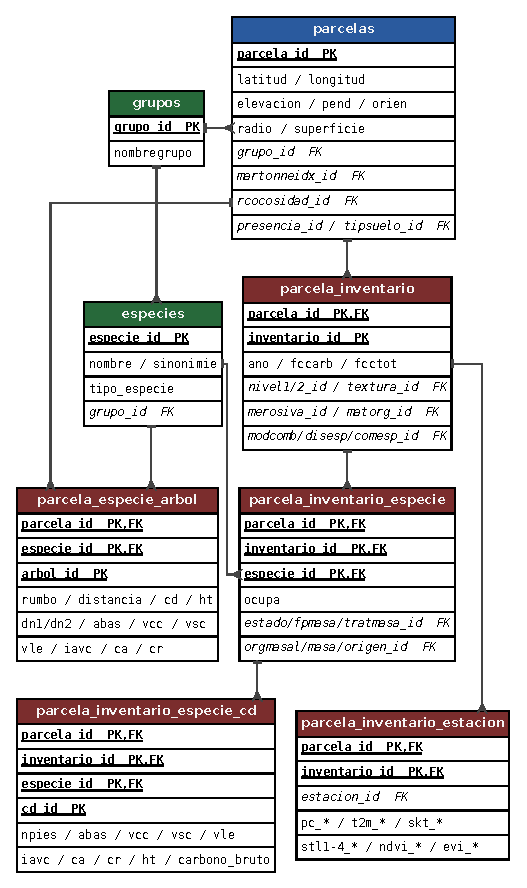
\includegraphics[width=\linewidth]{figuras/05_metodologia/er_diagram.pdf}
    \caption{Relational schema of the main database tables. Figure extracted from \cite{greenwestdb}, where further details on the variables can be found.}
    \label{fig:GWestBBDD}
\end{figure}


\subsection{Target variables}

The goal of the model is to estimate the \textbf{total carbon} that a forest plot will capture over a time horizon of 20--30 years, based on conditions observed in previous inventories.
Two complementary response variables are considered, both derived from the National Forest Inventory (IFN) data, allowing carbon content to be analysed from different perspectives: one normalised by area and another in absolute terms.


\begin{enumerate}
    \item \textbf{\texttt{c}} (tC/ha): represents the \textbf{total carbon contained in aboveground and belowground living biomass} per unit area, expressed in \emph{tonnes of carbon per hectare}.
          Its calculation is based on the sum of the aboveground (\texttt{ca}) and root (\texttt{cr}) carbon estimates reported by the IFN.
          In cases with missing values, the information was completed using a \emph{Random Forest Regressor} model fitted on observed dendrometric variables (Species, CD, VSC, NPies, ABas, IAVC, VCC and VLE), achieving satisfactory performance (\(R^2_{test} > 0.90\)).
          This variable is consistent with international forest inventory reporting formats and allows carbon content to be compared across plots or species.


    \item \textbf{\texttt{carbono\_bruto}} (tC): corresponds to the \textbf{total carbon captured per plot and species}, expressed in \emph{total tonnes of carbon}.
          Its estimation is performed in a traceable and physically interpretable manner from variables measured directly in the field: number of trees (\texttt{npies}), mean height (\texttt{ht}), species type (\texttt{clase\_especie}) and diameter class (\texttt{cd\_id}).
          The calculation follows an allometric model adapted from \cite{chave2014} and the IPCC guidelines~\cite{IPCC2006}, incorporating both aboveground and root biomass via the Root-to-Shoot ratio ($R$).
          The result is expressed in total tonnes of carbon per plot, without normalisation by area, which facilitates the traceability of the process and the comparison between inventories without depending on IFN-specific expansion factors.
          Consistent with the criteria for afforestation and reforestation projects, observations corresponding to seedlings or saplings are assigned a zero carbon value, since early development stages are not officially counted as captured carbon.
\end{enumerate}


These two variables summarise forest carbon content from complementary perspectives:
\texttt{c} (tC/ha) enables spatial and temporal comparison between forest stands, while \texttt{carbono\_bruto} (tC) provides an absolute measure directly derived from field observations.
Both constitute the main targets of the predictive modelling, aimed at estimating the carbon accumulated in \textbf{IFN4} from the conditions recorded in the previous inventories (\textbf{IFN2} and \textbf{IFN3}).

For further details on the origin of these variables, see \cite{greenwestdb}.

\subsection{Eligibility assumptions and external verification}
% Intervención humana, permanencia 30a (extrapolación cauta), superficie>=1ha,
% fccarb>=20% (filtro), altura>=3m en madurez (decisión de diseño).
As already introduced, for a forest project to be eligible for \emph{carbon credit} programmes in Spain, certain technical requirements must be met \cite{IPCC2006, miteco_guia_co2}. Each criterion and the way it is addressed in this study are summarised below:

\begin{itemize}
    \item \textbf{Direct human intervention.} The carbon increment must result from planned actions (reforestation, restoration or sustainable management). In our case, the model is trained on observational data (IFN2--IFN3--IFN4); therefore, \emph{intervention verification} is not inferred from the model, but is considered as an \emph{external condition} of eligibility for the project to be evaluated.

    \item \textbf{Minimum permanence.} The interval between IFN3 and IFN4 is mostly between 6 and 17 years (Figure~\ref{fig:periodo34}), a range too narrow for the 20--30 year reference horizon. To extend temporal coverage, the IFN2--IFN3 pair was also integrated, yielding intervals of 6 to 29 years (Figure~\ref{fig:periodo234}), more representative of the target horizon.

          \begin{figure}
              \centering
              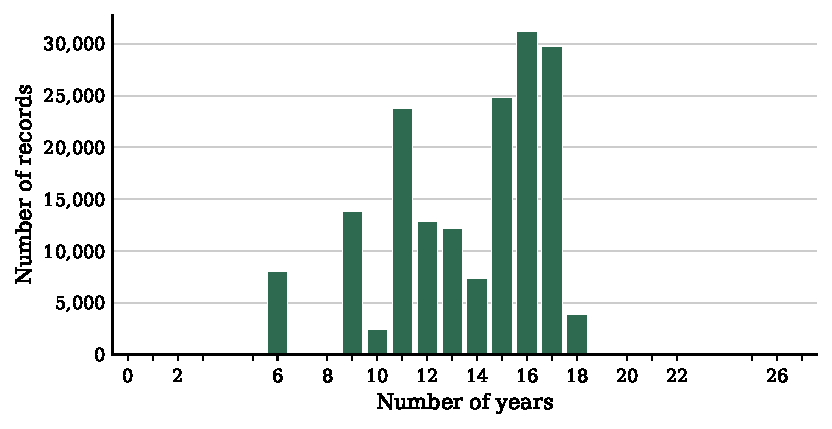
\includegraphics[width=\linewidth]{figuras/05_metodologia/hist_periodo_ifn34.pdf}
              \caption{Distribution of the year difference between the third and fourth inventories.}
              \label{fig:periodo34}
          \end{figure}

          \begin{figure}
              \centering
              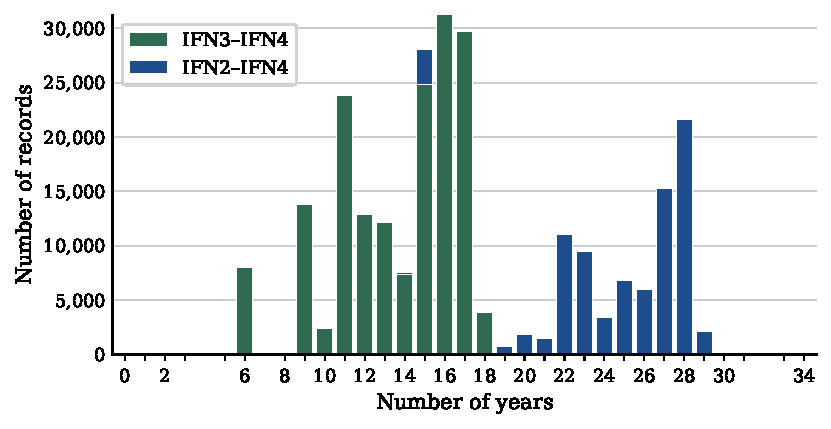
\includegraphics[width=\linewidth]{figuras/05_metodologia/hist_periodo.pdf}
              \caption{Distribution of the year difference between the IFN2--IFN3 and IFN3--IFN4 inventories.}
              \label{fig:periodo234}
          \end{figure}

    \item \textbf{Minimum area of 1 ha.} This is a criterion external to the model, verifiable \emph{ex ante} from the declared project geometry. In homogeneous stands, total carbon is approximately proportional to area, so this requirement does not affect model fitting.

    \item \textbf{Minimum canopy cover fraction of 20\%.} The database provides \texttt{fccarb} (tree canopy cover) and \texttt{fcctot} (total cover). This threshold is applied as an \emph{eligibility filter} prior to modelling ($\texttt{fccarb} \geq 20$).

    \item \textbf{Minimum height of 3 m at maturity.} This refers to the adult height of the species, not to the seedlings at the time of inventory. It is evaluated externally through the selection of appropriate species and does not intervene in model training.
\end{itemize}

\subsection{Data preparation and processing}
% Filtros (fccarb>=20%, crecimiento positivo, etc.)
% Agregaciones (parcela-especie, compresión CD -> npies_{cd}, etc.)
% Cálculo de variables derivadas (carbono\_bruto)
% Codificación y escalado

As already introduced, training is carried out along two lines according to the target variable: carbon in tonnes per hectare (\texttt{c} from \textbf{IFN4}) or carbon in tonnes (\texttt{carbono\_bruto} from \textbf{IFN4}); and according to the information used as explanatory variables: \textbf{IFN3} or \textbf{IFN3} and \textbf{IFN2}. Data preparation and filtering are presented in general terms.

\subsubsection{Record filtering}\label{subsec:filtradoregistros}

All plots in which the total carbon value (target variable) at the second inventory is lower than at the first are discarded. These cases are usually due to deforestation episodes, fires or other disturbances, and do not represent net forest growth.


The dataset is restricted to plots with a \texttt{fccarb} (tree canopy cover fraction) equal to or greater than 20\,\% in the explanatory inventory. This threshold defines the minimum proportion of area occupied by tree crowns relative to the total plot area, and constitutes one of the essential conditions for considering a surface as forest land. Excluding plots with \texttt{fccarb} below 20\,\% ensures that carbon estimates are made on consolidated forest stands, avoiding biases associated with agricultural areas or shrublands. The \textbf{IFN2} data are not subject to this filter because the \texttt{fccarb} variable is not available for that inventory.


\subsubsection{Variable calculation and aggregation}

Each input record is generated at the plot--species combination level, incorporating the corresponding variables from the first measurement and the target variable (carbon) from the second measurement (IFN4). The \texttt{parcela} and \texttt{parcela\_inventario} variables are split for each species. The entries in the \texttt{parcela\_inventario\_especie\_cd} table are grouped by plot and species and compressed into a single entry by creating a set of variables for each diameter class.


% La Tabla~\ref{tab:entradamodelo} resume las variables empleadas como entrada al modelo, integradas desde las distintas tablas que conforman la base de datos relacional.

% \begin{table*}
%     \renewcommand{\arraystretch}{1.2}
%     \setlength{\tabcolsep}{3pt}
%     \centering
%     \footnotesize
%     \resizebox{\textwidth}{!}{
%         \begin{tabular}{|p{3.2cm}|p{1.8cm}|p{6.5cm}|p{2.2cm}|}
%             \hline
%             \multicolumn{4}{|c|}{\textbf{Model Input Data Summary}}                                                                                                                                                                                                                                                                  \\
%             \hline
%             \textbf{Variable}                                                                                                                                                                 & \textbf{Type} & \textbf{Description}                              & \textbf{Annex}                                                                 \\
%             \hline
%             \textcolor{ForestGreen}{\texttt{parcela\_id}}                                                                                                                                     & varchar       & Unique plot identifier.                   & --                                                                             \\
%             \hline
%             \textcolor{ForestGreen}{\texttt{especie\_id}, \texttt{tipo\_especie}, \texttt{grupo\_id}}                                                                                         & int (CF)      & Species, type and taxonomic group.                 & \ref{sec:especies}, \ref{sec:gruposespecies}                                   \\
%             \hline
%             \textcolor{ForestGreen}{\texttt{ocupa}}                                                                                                                                           & int           & Occupancy degree (0--10).                       & --                                                                             \\
%             \hline
%             \textcolor{ForestGreen}{\texttt{estado\_id}}, \texttt{fpmasa\_id}, \texttt{tratmasa\_id}, \texttt{orgmasa1\_id}                                                                   & int (CF)      & State, stand form, treatment, organisation. & \ref{sec:EstadoIFN34}, \ref{sec:FPMasa}, \ref{sec:tratmasa}, \ref{sec:OrgMasa} \\
%             \hline
%             \textcolor{ForestGreen}{\texttt{tipsuelo1-3\_id}}                                                                                                                                 & int (CF)      & Soil types.                                   & Annex \ref{sec:TipSuelo}                                                       \\
%             \hline
%             \textcolor{ForestGreen}{\texttt{rocosidad\_id}}, \texttt{textura\_id}, \texttt{matorg\_id}, \texttt{modcomb\_id}, \texttt{disesp\_id}, \texttt{comesp\_id}, \texttt{merosiva\_id} & int (CF)      & Edaphic and structural variables.               & Various appendices                                                               \\
%             \hline
%             \textcolor{ForestGreen}{\texttt{radio}, \texttt{orientacion}, \texttt{elevacion}, \texttt{pendiente}}                                                                             & float         & Topography and plot geometry.                & --                                                                             \\
%             \hline
%             \textcolor{ForestGreen}{\texttt{martonneidx\_id}}                                                                                                                                 & int (CF)      & Martonne aridity index.                     & --                                                                             \\
%             \hline
%             \texttt{nivel1\_id}, \texttt{nivel2\_id}, \texttt{fccarb}, \texttt{fcctot}                                                                                                        & int/float     & Hierarchical levels and canopy cover.            & \ref{sec:nivel1}, \ref{sec:nivel2}                                             \\
%             \hline
%             \textcolor{ForestGreen}{\texttt{npies\_\{CD\}}}                                                                                                                                   & float         & Number of trees per diameter class.                 & --                                                                             \\
%             \hline
%             \textcolor{ForestGreen}{\texttt{periodo}}                                                                                                                                         & int           & Years between inventories.                           & --                                                                             \\
%             \hline
%             \textcolor{ForestGreen}{\texttt{evi, gndvi, ndii, ndvi\_\{stat\}\_\{est\}}}                                                                                                       & float         & Vegetation indices by season.               & --                                                                             \\
%             \hline
%             \textcolor{ForestGreen}{\texttt{pr, skt, stl1-4, t2m\_\{stat\}\_\{est\}}}                                                                                                        & float         & Climatic variables by season.                & --                                                                             \\
%             \hline
%             \textcolor{ForestGreen}{\texttt{c4}, \texttt{carbono\_bruto4}}                                                                                                                    & float         & IFN4 carbon (t/ha and t).                          & --                                                                             \\
%             \hline
%         \end{tabular}
%     }
%     \caption{Model input variables. Variables in \textcolor{ForestGreen}{green} are available in IFN2 and IFN3; the rest only in IFN3.}
%     \label{tab:entradamodelo}
% \end{table*}


\subsubsection{Reclassification of the \texttt{pendiente} and \texttt{orientacion} variables}

Since the ecological effect of slope and aspect on carbon accumulation is non-linear, both variables were reclassified as categorical factors. The \texttt{pendiente\_cat} variable was defined using seven intervals ($<5^\circ$, $5$--$10^\circ$, $10$--$15^\circ$, $15$--$20^\circ$, $20$--$30^\circ$, $30$--$50^\circ$, $>50^\circ$); the \texttt{orientacion\_cat} variable into eight equiangular cardinal sectors (\texttt{N}, \texttt{NE}, \texttt{E}, \texttt{SE}, \texttt{S}, \texttt{SO}, \texttt{O}, \texttt{NO}).

\subsubsection{Grouping of the \texttt{periodo} variable}

As can be seen in Figure~\ref{fig:periodo234}, the distribution of the \texttt{periodo} variable, defined as the number of years elapsed between the measurement of the explanatory variables and the observation of the target variable, shows some heterogeneity in its frequency. Although the total range of values extends approximately between 0 and 34 years, some temporal intervals are represented by a very small number of observations.

This scarcity of data for certain values of \texttt{periodo} can introduce instability in model training, by forcing the algorithm to learn patterns from poorly representative samples. To mitigate this effect and improve the robustness of predictions, certain values of \texttt{periodo} were grouped into broader temporal categories, giving rise to a new variable called \texttt{periodo\_agrupado}.

The grouping procedure was designed conservatively, keeping unchanged those values with sufficient sample support and grouping only the most scarce intervals. Specifically, values below 6 years were grouped into category 5; periods between 7 and 10 years were grouped into 10; those between 18 and 21 years were grouped into 20; and values equal to or greater than 29 years were grouped into 30. The remaining intermediate values were left unchanged.

It should be noted that the \texttt{periodo\_agrupado} variable does not retain the full granularity of the original variable, but does retain its essential temporal meaning. The experiments carried out show that this representation is more statistically stable and leads to models with more robust predictive behaviour, by reducing sensitivity to temporal intervals with low observation frequency.

\subsection{Partitioning and validation}

To obtain an unbiased estimate of performance and avoid \emph{data leakage} arising from the hierarchical structure of the data, the training process is organised at two levels: (i) an external \emph{hold-out} partition for final evaluation and (ii) an internal cross-validation for hyperparameter selection.

\noindent\textbf{Train/test split.} The filtered data are split into 80\% for training and 20\% for test. This split is made so that all observations associated with the same plot are assigned entirely to one of the subsets.

\noindent\textbf{Cross-validation for hyperparameter selection.} Hyperparameter selection is carried out exclusively on the training set using \texttt{GridSearchCV} with $R^2$ as the optimisation metric. \texttt{GroupKFold} with $k=5$ folds is used, ensuring there is no overlap of plots between folds (i.e., the grouping is respected both in the hold-out and in the internal validation).

\vspace{0.25em}
\vspace{0.25em}
\noindent\textbf{Evaluation metrics.} The main metrics used are RMSE, RMSE\%, $R^2$, MAE and SMAPE. In the following expressions, $y_i$ is the observed value, $\hat{y}_i$ the predicted value, $\bar{y}$ the observed mean and $n$ the number of observations:

\begin{itemize}
    \item \textbf{RMSE:} root mean squared error, in the same units as the target variable.
          \begin{equation}
              \text{RMSE} = \sqrt{\frac{1}{n} \sum_{i=1}^{n} (y_i - \hat{y}_i)^2}
          \end{equation}

    \item \textbf{RMSE\%:} RMSE expressed as a percentage of the observed mean.
          \begin{equation}
              \text{RMSE}_{\%} = \frac{\text{RMSE}}{\bar{y}} \times 100
          \end{equation}

    \item \textbf{MAE} (mean absolute error): average of absolute errors; more robust than RMSE against outliers by penalising all residuals equally.
          \begin{equation}
              \text{MAE} = \frac{1}{n} \sum_{i=1}^{n} |y_i - \hat{y}_i|
          \end{equation}

    \item \boldmath\textbf{$R^2$}\unboldmath{} \textbf{(coefficient of determination):} proportion of variance explained by the model.
          \begin{equation}
              R^2 = 1 - \frac{\sum_{i=1}^{n} (y_i - \hat{y}_i)^2}{\sum_{i=1}^{n} (y_i - \bar{y})^2}
          \end{equation}

    \item \textbf{SMAPE:} symmetric percentage error, bounded and robust against the asymmetry of MAPE.
          \begin{equation}
              \text{SMAPE} = \frac{100}{n} \sum_{i=1}^{n} \frac{|y_i - \hat{y}_i|}{(|y_i| + |\hat{y}_i|)/2}
          \end{equation}
\end{itemize}

As supporting metrics for residual analysis and bias detection, MAE, MAPE, wMAPE, MedAE and Bias are also calculated.

%\vspace{0.25em}
%\noindent\textbf{Reporting protocol.} For each model the following are reported: (i) mean performance and dispersion in group cross-validation (training), and (ii) final performance on the independent evaluation set (20\,\%). This protocol guarantees comparability between models, control of spatial bias by plot and explicit verification of temporal robustness.

\subsubsection{Encoding and normalisation}

In order to ensure methodological consistency and avoid \emph{data leakage} during cross-validation, all preprocessing steps are explicitly integrated inside a \texttt{Pipeline} together with the regression model. In this way, the parameters associated with preprocessing are estimated \emph{exclusively} from the training data of each fold, and subsequently applied to the validation or test data.

Variables are treated according to their nature:

\begin{itemize}
    \item \textbf{Continuous numerical variables}: imputed using the median to reduce the influence of extreme values and subsequently standardised via \emph{z-score} normalisation (zero mean and unit standard deviation). This step is especially relevant for models sensitive to variable scale, such as linear regressions, SVR or neural networks.

    \item \textbf{Density structural variables} (\texttt{npies\_*}): as they represent counts per diameter class, they are imputed with zero when absent and standardised in the same way as numerical variables, preserving their relative contribution in the model.

    \item \textbf{Categorical variables}: imputed using the mode, explicitly converted to string type and encoded via \textit{one-hot encoding}. The \texttt{handle\_unknown='ignore'} option is used to ensure the model's robustness against categories not observed during training.
\end{itemize}

This strategy ensures that the encoding, imputation and scaling of variables are performed consistently across all evaluated models and that the estimated performance faithfully reflects the system's generalisation capacity, without introducing biases derived from improper access to information from the evaluation set.

\subsection{Feature selection}

Predictor selection combined automatic methods and expert criteria. Among the automatic methods, \textit{Featurewiz} was used, which eliminates predictors with high correlation ($|r|>0.70$) and refines the selection via \textit{Gradient Boosting}, and \textit{mRMR} (minimum Redundancy--maximum Relevance), which maximises the relevance of each predictor with respect to the target while minimising redundancy among them via mutual information.

These results were integrated with a manual selection based on statistical (correlations, ANOVA, redundancy analysis) and ecological criteria, guaranteeing the representation of the essential dimensions of the system (stand structure, topography, soil, climate and spectral indices). Additionally, a supervised sequential procedure (SSSRP) of \textit{forward selection} was applied on a CatBoost model, incorporating at each iteration the variable with the greatest gain in $R^2$ until $\Delta R^2 < 10^{-5}$ was reached. The final result was a set of 44 variables selected from 445 candidates.

\subsection{Evaluated models}\label{subsec:modelosevaluados}

Nine representative algorithms from different paradigms were evaluated: \textit{boosting} methods (XGBoost, LightGBM, CatBoost, GBDT), \textit{bagging} methods (Random Forest, BaggedDT) and reference models (SVR, MLP, BayesianNN). Their main characteristics are summarised in Table~\ref{tab:modelos}. The best base models were subsequently combined in \textit{stacking} configurations.

\subsubsection{\textit{Stacking} configuration}

After evaluating all the above models, different base learner configurations were built that are combined via a meta-model. These combinations were designed according to two main criteria:

\begin{enumerate}
    \item \textbf{Structural diversity:} mixing boosting and bagging methods, as well as boosting variants with different growth strategies and regularisation.
    \item \textbf{Individual performance:} preferentially including models with higher $R^2$ and lower error (RMSE, MAE) in individual tests.
\end{enumerate}

The meta-models used to integrate the predictions were:

\begin{itemize}
    \item \textbf{Linear models:} Linear Regression, Ridge.
    \item \textbf{Tree-based models:} Random Forest, Gradient Boosting Regressor.
    \item \textbf{Kernel models:} Linear SVR.
    \item \textbf{Neural network:} MLP with one hidden layer.
\end{itemize}

This selection allows comparison from simple linear combiners to non-linear integrators capable of capturing complex interactions between predictions.

\subsubsection{Model comparison and justification}

The exhaustive evaluation of multiple algorithms allows identifying not only the best-performing individual model, but also synergistic combinations for \textit{stacking}. Table~\ref{tab:modelos} summarises the models finally trained and evaluated.


\begin{table*}[htbp]
    \centering
    \footnotesize
    \resizebox{\textwidth}{!}{
        \begin{tabular}{llll}
            \toprule
            \textbf{Model} & \textbf{Type}  & \textbf{Characteristics}                       & \textbf{Notes}         \\
            \midrule
            Random Forest   & Bagging        & Bootstrap with random feature selection & Robust and stable              \\
            BaggedDT        & Bagging        & Unpruned trees on bootstrap samples      & Improvement by aggregation          \\
            XGBoost         & Boosting       & L1/L2 regularisation, second order            & Very accurate; sensitive to tuning \\
            LightGBM        & Boosting       & Leaf-wise growth, very efficient           & Fast; risk of overfitting  \\
            CatBoost        & Boosting       & Ordered encoding; robust to noise        & Excellent without extensive tuning      \\
            GBDT            & Boosting       & Sequential trees fitted to residuals      & Good performance               \\
            MLP             & Neural network   & Captures non-linear relationships                 & Requires normalisation         \\
            SVR             & Margin-based       & Linear kernel, large margin                     & Robust against overfitting         \\
            BayesianNN      & Probabilistic & Quantifies uncertainty                       & Reduces overfitting             \\
            \bottomrule
        \end{tabular}
    }
    \caption{Supervised learning models evaluated.}
    \label{tab:modelos}
\end{table*}



